%!TEX root=../protocol.tex	% Optional

\section{Naměřené hodnoty}

\subsection{Data závislosti útlumu na podélném vychýlení optických kabelů}

\begin{table}[h!]

%\captionsetup{justification=raggedright,singlelinecheck=false, margin={1.5cm,0cm}} % Move caption to the left
\caption{Pro čelní vzdálenost vláken 5 mm }
\centering
\begin{tabular}{ | c | c | c | } 
  \hline
  vzdálenost / mm & výkon / $\mu$W & optický výkon / dBm  \\ 
     \hline
   1 & 21,1 & -10,8\\ 
     \hline
   2 & 12,6 & -12,5\\ 
     \hline
   3 & 7,0 & -15,5\\ 
     \hline
   4 & 4,9 & -17,4\\ 
     \hline
   5  & 3,1 & -19,24\\ 
     \hline
   6  & 2,6 & -20,1\\ 
     \hline
   7  & 1,7 & -21,9\\ 
     \hline
   8  & 1,64 & -23,0\\ 
     \hline
   9  & 1,32 & -23,6\\ 
     \hline
   10  & 0,94 & -24,3\\ 
     \hline
   15  & 0,43 & -27,2\\ 
     \hline
   20  & 0,25 & -30,5\\ 
     \hline
   25  & 0,17 & -32,7\\ 
     \hline
   30  & 0,10 & -33,9\\ 
     \hline
   35 & 0,09 & -35,6\\ 
     \hline
\end{tabular}
\label{table:1}
\end{table}

\begin{figure}[h]
\centering
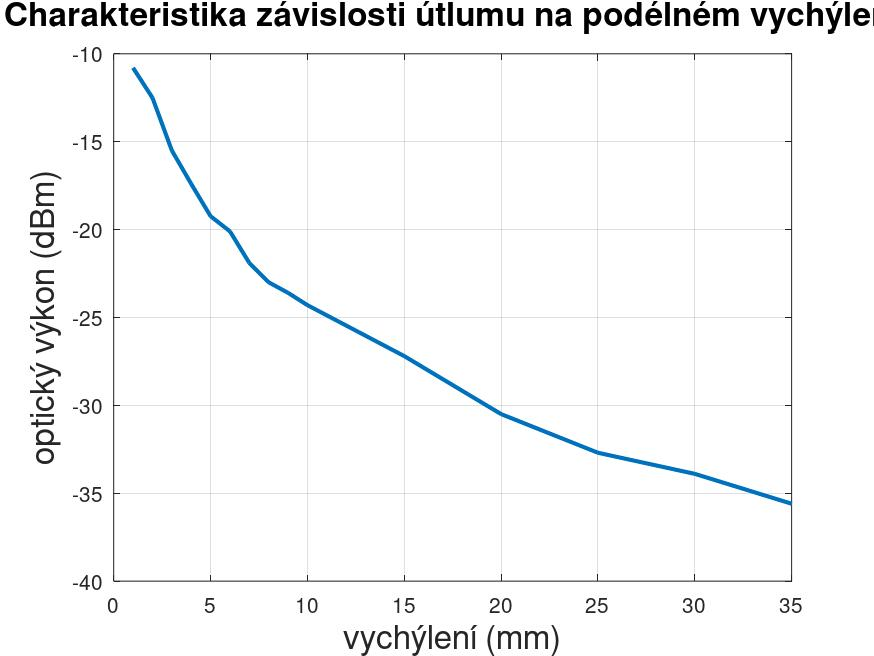
\includegraphics[width=11cm]{images/plot2.jpg}
\caption{}
\label{fig:12}
\end{figure}


\newpage

\subsection{Data měření závislosti útlumu na úhlovém vychýlení optických konektorů}

\begin{table}[!htb]
    %\caption{Závislost útlumu na příčném vychýlení optických konektorů}
    \begin{minipage}{.5\linewidth}
      \caption{Pro čelní vzdálenost vláken 5 mm}
      \centering
        \begin{tabular}{| c | c |}
  \hline
  úhel vychýlení / \textdegree & výkon / $\mu$W  \\ 
     \hline
  -25 & 0,144 \\ 
     \hline
  -20 & 0,310 \\ 
     \hline
  -15 & 0,780 \\
     \hline
  -10 & 1,470 \\ 
     \hline
   -5 & 1,920 \\ 
     \hline
   0 & 2,130 \\  
     \hline
   5 & 1,840 \\ 
     \hline
   10 & 1,290 \\ 
     \hline
   15 & 0,650 \\ 
     \hline
   20 & 0,440 \\ 
     \hline
   25 & 0,103 \\ 
     \hline

        \end{tabular}
    \end{minipage}%
    \begin{minipage}{.5\linewidth}
      \centering
        \caption{Závislost výkonu na úhlu natočení}
        \begin{tabular}{| c | c |}
     \hline
    úhel vychýlení / \textdegree & množství přeneseného výkonu / \%  \\
     \hline
  -25 & 6,76 \\ 
     \hline
  -20 & 14,55 \\ 
     \hline
  -15 & 36,62 \\
     \hline
  -10 & 69,01 \\ 
     \hline
   -5 & 90,14 \\ 
     \hline
   0 & 100 \\  
     \hline
   5 & 86,39 \\ 
     \hline
   10 & 60,56 \\ 
     \hline
   15 & 30,52 \\ 
     \hline
   20 & 20,66 \\ 
     \hline
   25 & 4,84 \\ 
     \hline
        \end{tabular}
    \end{minipage} 
\end{table}

\begin{figure}[h]
\centering
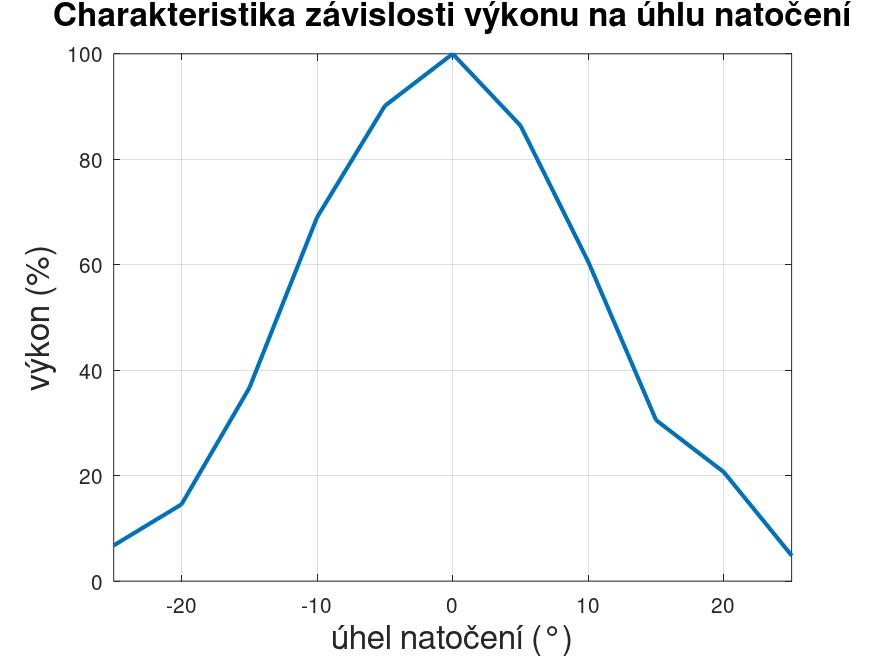
\includegraphics[width=11cm]{images/plot.jpg}
\caption{}
\label{fig:13}
\end{figure}

\newpage
\subsection{Stanovení numerické aparatury}

Když $n_1 = 1,49$ a $n_2 = 1,41$, pak $NA = \sqrt{1,49^2 - 1,41 ^ 2}$ $\dot{=}$ $0,482$.
\\\\
Při měření jsme zjistili, že když je úhel vychýlení -25\textdegree, tak je množství přeneseného signálu \mbox{6,76 \%}.
Odhadem se dá tedy říct, že zhruba při -28\textdegree \ bude výkon roven teoretické numerické aparatuře. 

\newpage
\subsection{Data měření závislosti útlumu na příčném vychýlení optických konektorů}

\begin{table}[!htb]
    %\caption{Závislost útlumu na příčném vychýlení optických konektorů}
    \begin{minipage}{.5\linewidth}
      \caption{Čelní vzdálenost vláken 5 mm}
      \centering
        \begin{tabular}{| c | c |}
     \hline
    úhel vychýlení / \textdegree & optický výkon / dBm  \\ 
     \hline
  -5 & -$\infty$ \\ 
     \hline
  -4,5 & -$\infty$ \\ 
     \hline
  -4 & -$\infty$ \\
     \hline
  -3,5 & -$\infty$ \\ 
     \hline
   -3 & -$\infty$ \\ 
     \hline
   -2,5 & -41,32 \\  
     \hline
   -2 & -36,65 \\ 
     \hline
   -1,5 & -34,55 \\ 
     \hline
   -1 & -32,85 \\ 
     \hline
   -0,5 & -31,23 \\ 
     \hline
   0 & -30,74 \\ 
     \hline
   0,5 & -30,40 \\ 
     \hline
   1 & -31,11 \\ 
     \hline
   1,5 & -32,28 \\ 
     \hline
   2 & -33,44 \\ 
     \hline
   2,5 & -36,32 \\  
     \hline
   3 & -38,84 \\ 
     \hline
  3,5 & -$\infty$ \\ 
     \hline
  4 & -$\infty$ \\
     \hline
  4,5 & -$\infty$ \\ 
     \hline
  5 & -$\infty$ \\ 
     \hline
        \end{tabular}
    \end{minipage}%
    \begin{minipage}{.5\linewidth}
      \centering
        \caption{Čelní vzdálenost vláken 10 mm}
        \begin{tabular}{| c | c |}
     \hline
    úhel vychýlení / \textdegree & optický výkon / dBm  \\ 
     \hline
  -5 &  -41,85 \\ 
     \hline
  -4,5 & -41,18 \\ 
     \hline
  -4 & -40,19 \\
     \hline
  -3,5 & -39,14 \\ 
     \hline
   -3 & -38,25 \\ 
     \hline
   -2,5 & -37,43 \\  
     \hline
   -2 & -36,74 \\ 
     \hline
   -1,5 & -36,21 \\ 
     \hline
   -1 & -35,78 \\ 
     \hline
   -0,5 & -35,49 \\ 
     \hline
   0 & -35,30 \\ 
     \hline
   0,5 & -35,43 \\ 
     \hline
   1 & -35,58 \\ 
     \hline
   1,5 & -35,77 \\ 
     \hline
   2 & -36,24 \\ 
     \hline
   2,5 & -36,80 \\  
     \hline
   3 & -37,20 \\ 
     \hline
  3,5 & -38,20 \\ 
     \hline
  4 & -38,21 \\
     \hline
  4,5 & -39,12 \\ 
     \hline
  5 & -40,49 \\ 
     \hline
        \end{tabular}
    \end{minipage} 
\end{table}

\newpage
\subsection{Využití střídavého optického signálu}

Především kvůli vnějšímu rušení. Například sluneční svit by mohl ovlivnit přesun dat svou frekvencí, proto je potřeba se odlišit výrazně jinou frekvencí signálu.
\\\\
Střídavý signál má zároveň větší použitelný dosah oproti stejnosměrnému, protože se dá snadněji zesilovat. 


\subsection{Závislost útlumu na ohnutí optického kanálu}

\begin{table}[h!]

%\captionsetup{justification=raggedright,singlelinecheck=false, margin={1.5cm,0cm}} % Move caption to the left
\caption{Pro čelní vzdálenost vláken 5 mm }
\centering
\begin{tabular}{ | c | c | c | c | } 
  \hline
  poloměr / cm & výkon / $\mu$W & optický výkon / dBm  \\ 
     \hline
  4 & 15,3 & -12,30\\ 
     \hline
  5 & 14,6 & -12,41\\ 
     \hline
  6 & 15,1 & -12,65\\
     \hline
\end{tabular}
\label{table:4}
\end{table}

\subsection{Spektrální závislost útlumu optických vláken}

\begin{table}[!htb]
    %\caption{Závislost útlumu na příčném vychýlení optických konektorů}
    \begin{minipage}{.5\linewidth}
      \caption{Optický kabel délky 1 m}
      \centering
        \begin{tabular}{| c | c |}
     \hline
    vlnová délka / nm & optický výkon / dBm  \\ 
     \hline
  526 & -19,28 \\ 
     \hline
  560 & -22,50 \\ 
     \hline
  660 & -12,10 \\
     \hline
  850 & -31,11 \\ 
     \hline

        \end{tabular}
    \end{minipage}%
    \begin{minipage}{.5\linewidth}
      \centering
        \caption{Optický kabel délky 50 m}
        \begin{tabular}{| c | c |}
     \hline
    vlnová délka / nm & optický výkon / dBm  \\ 
     \hline
  526 & -29,38 \\ 
     \hline
  560 & -34,09 \\ 
     \hline
  660 & -25,83 \\
     \hline
  850 & -$\infty$ \\ 
     \hline
        \end{tabular}
    \end{minipage} 
\end{table}

\subsection{Barevný posun světla}
Konec vlákna jsme nastavili směrem k svítilně v mobilním telefonu. Na druhém konci jsme viděli tyrkysové světlo. 
\\\\
Průchod tyrkysového světla optickým vláknem je pravděpodobně způsoben fyzikálními vlastnostmi materiálu, ze kterého je vlákno vyrobeno. Tyrkysová vlnová délka je možná ta, která nejefektivněji prochází tímto konkrétním materiálem s nejmenšími ztrátami. Optická vlákna jsou navržena tak, aby minimalizovala ztráty světla při přenosu a aby co nejlépe využila vlastnosti materiálu pro propagaci světla. Tyrkysová barva na konci optického vlákna by tak mohla naznačovat optimální propustnost tohoto materiálu právě pro tuto konkrétní vlnovou délku světla.



\newpage
\section{Zhodnocení}
Během měření jsme ověřili útlumové vlastnosti přenosu optickým vláknem. Všechny hodnoty vycházely dle předpokladů, s ohledem na chyby zavedené manuálním měřením vzdáleností. Při měření spektrální závislosti útlumu na optických vláknech při vlnové délce 850 nm a 50 metrovém kabelu jsme již nebyli schopni změřit optický výkon, kvůli silnému útlumu vlákna. Bohužel už nezbyl čas na doměření závislosti alespoň s 2 metrovým kabelem.
\\\\
Přenos WDM signálu nebyl měřen pro nedostatek času.
\\\\
Během měření jsme si ověřili některé vlastnosti optických vláken, například, že s rostoucím oddálením konektorů dvou vláken od sebe se exponenciálně snižuje optický výkon vláknem.
